\documentclass[9pt]{beamer}
\mode<presentation>

\usetheme{Madrid}
\usecolortheme[RGB={65,27,214}]{structure}
\usefonttheme{structurebold}
\setbeamercovered{invisible}

\usepackage{dynblocks}
\usepackage{textpos}
\usepackage{amsfonts}
\usepackage{amsmath}
\usepackage{amssymb}
\usepackage{amsthm}
\usepackage{mathtools}
\usepackage{hyperref}
\usepackage[utf8]{inputenc}
\usepackage[T1]{fontenc}
\usepackage{booktabs}
\usepackage{array}
\usepackage{colortbl}
\usepackage{authblk}
\usepackage{etoolbox}
\usepackage{lmodern}
\usepackage{eso-pic}
\usepackage{graphicx}
\usepackage{tikz}
\usetikzlibrary{arrows.meta, positioning, fit, backgrounds}

\makeatletter
\patchcmd{\@maketitle}{\LARGE \@title}{\fontsize{16}{19.2}\selectfont\@title}{}{}
\makeatother

\renewcommand\Authfont{\fontsize{12}{14.4}\selectfont}
\renewcommand\Affilfont{\fontsize{9}{10.8}\itshape}

\title[Diffusion for Inverse Problems]{Diffusion-Based Methods for Inverse Problems in Physical Data}

\author[Abdullaeva, Efimov, Losev, Sadreev]{%
  \textbf{Students}\\[0.2em]
  Mariia Abdullaeva \and Andrei Efimov \and Anton Losev \and Amir Sadreev}

\institute[Skoltech]{Skolkovo Institute of Science and Technology\\Deep Learning Final Project}

\titlegraphic{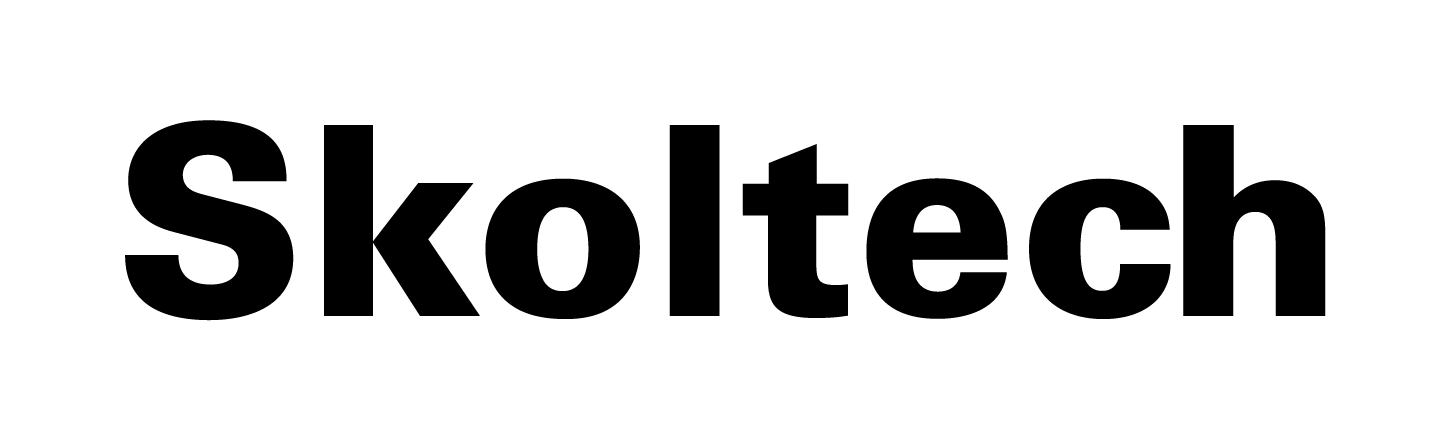
\includegraphics[width=4cm]{Logo.png}}
\date{}

% ─────────────────────────────────────────────────────────────
\begin{document}
% ─────────────────────────────────────────────────────────────

\begin{frame}[plain]
\begin{center}
\vspace*{1.0cm}
\begin{beamercolorbox}[sep=8pt,center,rounded=true,shadow=true]{title}
  {\usebeamerfont{title}\inserttitle\par}
\end{beamercolorbox}
\vspace{1.0cm}
Skolkovo Institute of Science and Technology\\
Deep Learning Final Project\\[0.35cm]
\makebox[\textwidth][r]{%
  \begin{tabular}{@{}l@{}}
  {\scriptsize\textbf{Students:} Mariia Abdullaeva, Andrei Efimov,}\\
  {\scriptsize\hspace{4.7em}Anton Losev, Amir Sadreev}
  \end{tabular}}
\vspace{0.35cm}

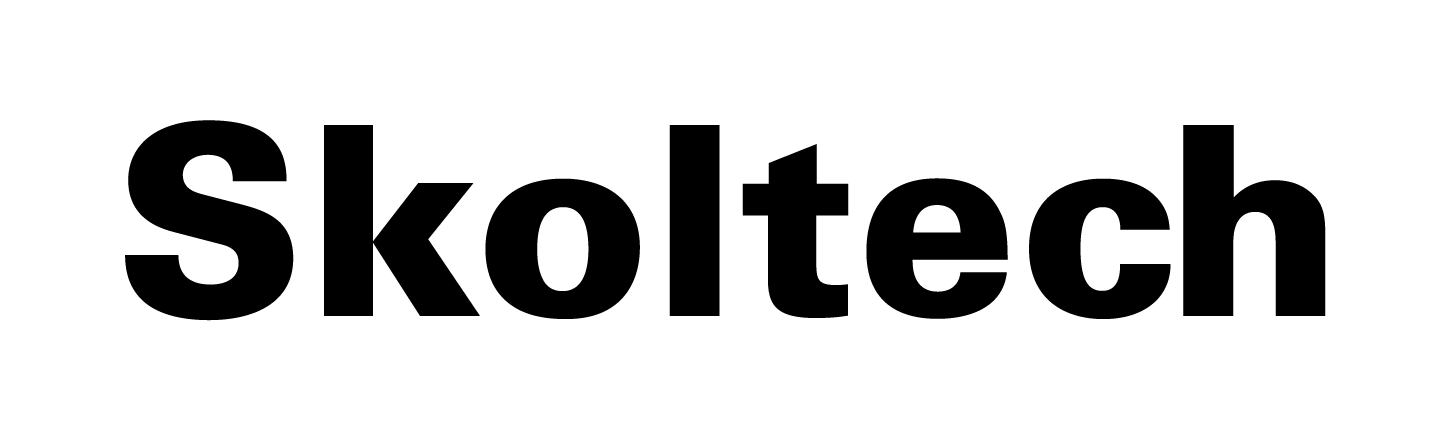
\includegraphics[width=4cm]{Logo.png}\\[0.4cm]
{\scriptsize\texttt{\href{https://github.com/mabdllv/DL_final_project}{\textcolor{blue}{github.com/mabdllv/DL\_final\_project}}}}
\end{center}
\end{frame}

\begin{frame}{Outline}
  \tableofcontents
\end{frame}

% ═════════════════════════════════════════════════════════════
\section{Introduction \& Motivation}
% ═════════════════════════════════════════════════════════════

\begin{frame}{Inverse Problems in Physics}
\begin{block}{The core challenge}
In many physical systems the full state $\mathbf{u}$ cannot be measured directly.
Sensors are sparse, expensive, or obscured.
We observe only
\[
  \mathbf{y} = A(\mathbf{u}) + \boldsymbol{\eta},
\]
and must recover the full field $\mathbf{u}$ from incomplete, possibly noisy data.
\end{block}
\begin{block}{Practical examples}
\begin{itemize}
  \item \textbf{Fluid dynamics:} PIV measurements give velocity at a sparse grid; the rest of the flow field is unknown.
  \item \textbf{Meteorology:} weather stations cover a tiny fraction of the atmosphere.
  \item \textbf{Medical imaging:} MRI/CT measure a transform of the tissue density, not density itself.
\end{itemize}
\end{block}
\begin{block}{Why is it hard?}
The problem is ill-posed: many fields $\mathbf{u}$ are consistent with the same observation $\mathbf{y}$.
A good reconstruction method must encode a \emph{prior} over physically realistic fields.
\end{block}
\end{frame}

% ─────────────────────────────────────────────────────────────

\begin{frame}{Classical Approaches and Their Limits}
\begin{block}{Standard baselines}
\begin{itemize}
  \item \textbf{Interpolation} (bilinear, RBF): cheap, but ignores global structure and physical constraints.
  \item \textbf{Variational / PDE-based methods}: require hand-crafted regularisers and domain knowledge.
  \item \textbf{Compressed sensing}: requires sparsity in a fixed basis; struggles with complex turbulent fields.
\end{itemize}
\end{block}
\begin{block}{What is missing}
\begin{itemize}
  \item No uncertainty quantification — outputs a single point estimate.
  \item Prior is fixed by hand, not learned from data.
  \item Cannot adapt to different observation operators without redesign.
\end{itemize}
\end{block}
\begin{alertblock}{Our approach}
Use a \textbf{diffusion model} trained on clean physical fields as a \emph{data-driven prior}.
At inference time, measurement guidance steers the sampling toward reconstructions that are
both physically plausible \emph{and} consistent with the observations.
No retraining is needed when $A$ changes.
\end{alertblock}
\end{frame}

% ─────────────────────────────────────────────────────────────

\begin{frame}{Project Scope and Goals}
\begin{block}{Setting}
\begin{itemize}
  \item \textbf{Data:} 2D Kolmogorov flow — a canonical turbulent velocity field $(u_x, u_y)$.
  \item \textbf{Task:} single-state reconstruction (not forecasting).
  \item \textbf{Operators $A$:} four representative types (sparse, masked, downsampled, blurred).
\end{itemize}
\end{block}
\begin{block}{Methods evaluated}
\begin{enumerate}
  \item \textbf{DDNM} — null-space decomposition for linear operators.
  \item \textbf{DPS} — gradient-guided posterior sampling (general differentiable $A$).
  \item \textbf{RePaint} — observation pasting for inpainting.
  \item \textbf{DDRM} — spectral decomposition via SVD/Fourier.
\end{enumerate}
\end{block}
\begin{block}{Physics constraint}
Incompressibility $\nabla \cdot \mathbf{u} = 0$ is enforced via Helmholtz projection during sampling,
at zero additional training cost.
\end{block}
\end{frame}

% ═════════════════════════════════════════════════════════════
\section{Background: Diffusion Models}
% ═════════════════════════════════════════════════════════════

\begin{frame}{Score-Based Diffusion: Forward Process}
\begin{block}{Variance-Preserving SDE (VP-SDE)}
Clean field $\mathbf{x}_0$ is gradually corrupted by adding Gaussian noise:
\[
  \mathbf{x}_t = \mu_t\,\mathbf{x}_0 + \sigma_t\,\boldsymbol{\varepsilon},
  \qquad \boldsymbol{\varepsilon} \sim \mathcal{N}(0, I),
\]
with schedule
\[
  \mu_t = \cos(\omega t), \qquad \sigma_t = \sqrt{1 - \mu_t^2}.
\]
At $t=0$: $\mathbf{x}_0$ is the clean field. At $t=T$: $\mathbf{x}_T \approx \mathcal{N}(0, I)$.
\end{block}
\begin{block}{Score function}
The score $\nabla_{\mathbf{x}_t}\log p_t(\mathbf{x}_t)$ parameterises the reverse process.
We train a neural network $\boldsymbol{\varepsilon}_\theta(\mathbf{x}_t, t)$ to predict the noise $\boldsymbol{\varepsilon}$,
which is equivalent to learning the score:
\[
  \mathcal{L} = \mathbb{E}_{t,\mathbf{x}_0,\boldsymbol{\varepsilon}}\bigl\|\boldsymbol{\varepsilon}_\theta(\mathbf{x}_t, t) - \boldsymbol{\varepsilon}\bigr\|^2.
\]
\end{block}
\end{frame}

% ─────────────────────────────────────────────────────────────

\begin{frame}{Score-Based Diffusion: Reverse Process}
\begin{block}{Deterministic reverse sampler}
Starting from $\mathbf{x}_T \sim \mathcal{N}(0, I)$, iterate from $t = T$ to $0$:
\begin{enumerate}
  \item Predict clean field: $\displaystyle\hat{\mathbf{x}}_0 = \frac{\mathbf{x}_t - \sigma_t\,\boldsymbol{\varepsilon}_\theta(\mathbf{x}_t, t)}{\mu_t}$.
  \item Step to next time: $\mathbf{x}_{t-1} = \mu_{t-1}\hat{\mathbf{x}}_0 + \sigma_{t-1}\,\boldsymbol{\varepsilon}_\theta(\mathbf{x}_t, t)$.
\end{enumerate}
\end{block}
\begin{block}{Why diffusion for inverse problems?}
\begin{itemize}
  \item The learned prior covers the entire distribution of realistic fields.
  \item Conditional sampling can be plugged in at inference time
        without modifying the score model.
  \item Multiple samples yield a distribution over plausible reconstructions.
\end{itemize}
\end{block}
\begin{block}{Key idea for conditional sampling}
At each reverse step, after computing $\hat{\mathbf{x}}_0$,
\textbf{inject measurement information} to enforce $A(\hat{\mathbf{x}}_0) \approx \mathbf{y}$.
Different methods differ in how this injection is done.
\end{block}
\end{frame}

% ═════════════════════════════════════════════════════════════
\section{Dataset \& Model}
% ═════════════════════════════════════════════════════════════

\begin{frame}{Kolmogorov Flow Dataset}
\begin{block}{Physical setup}
Kolmogorov flow: 2D incompressible Navier-Stokes with periodic forcing.
\[
  \partial_t \boldsymbol{\omega} + (\mathbf{u}\cdot\nabla)\boldsymbol{\omega}
    = \nu\,\Delta\boldsymbol{\omega} + f, \qquad f = A\sin(k_f y).
\]
Simulation in vorticity form on a periodic $256\times256$ grid.
\end{block}
\begin{block}{Dataset construction}
\begin{itemize}
  \item Velocity field $(u_x, u_y)$ computed from vorticity via stream function.
  \item Average-pooled to $64\times64$: tensor shape $[N, 2, 64, 64]$.
  \item Stored as \texttt{.npz} with metadata: \texttt{viscosity}, \texttt{drag}, \texttt{forcing\_amp}, \texttt{split}.
  \item Splits: \textbf{train} / \textbf{val} / \textbf{test} by trajectory ID.
\end{itemize}
\end{block}
\begin{block}{Normalisation}
\[
  \mathbf{x}_\text{norm} = \frac{\mathbf{x}_\text{raw} - \mu_\text{train}}{\sigma_\text{train}}.
\]
All sampling runs in normalised space; metrics are computed in raw velocity space.
\end{block}
\end{frame}

% ─────────────────────────────────────────────────────────────

\begin{frame}{Score Model Architecture}
\begin{block}{Model}
VP-SDE score network: \texttt{diffusers.UNet2DModel} with
\begin{itemize}
  \item \textbf{Circular padding} to respect periodic boundary conditions.
  \item \textbf{Fourier coordinate channels}: $\sin(x), \cos(x), \sin(y), \cos(y)$ appended to input.
    These are clean conditioning channels — they are not noised and do not enter the loss.
  \item Input: $[\mathbf{x}_t,\, \sin x,\, \cos x,\, \sin y,\, \cos y]$, 6 channels total.
\end{itemize}
\end{block}
\begin{block}{Training objective}
\[
  \mathcal{L} = \mathbb{E}_{t, \mathbf{x}_0, \boldsymbol{\varepsilon}}
    \bigl\|\boldsymbol{\varepsilon}_\theta\bigl(\mathbf{x}_t, t\bigr) - \boldsymbol{\varepsilon}\bigr\|^2.
\]
Noise schedule: cosine VP-SDE. Checkpoint saves \texttt{mean} and \texttt{std} for normalisation.
\end{block}
\begin{block}{Unconditional sampling quality}
The trained prior generates velocity snapshots that are visually and statistically
indistinguishable from held-out Kolmogorov fields. Divergence $\|\nabla\cdot\mathbf{u}\|$ of
prior samples is small but not exactly zero — physics constraint is added separately.
\end{block}
\end{frame}

% ─────────────────────────────────────────────────────────────

\begin{frame}{Model Architecture \& Training Setup}
\begin{block}{UNet architecture (\texttt{diffusers.UNet2DModel})}
\renewcommand{\arraystretch}{1.15}
\begin{center}
\begin{tabular}{ll}
\toprule
\textbf{Property} & \textbf{Value} \\
\midrule
Input channels & 6 \;($u_x, u_y$ noisy + $\sin x, \cos x, \sin y, \cos y$ clean) \\
Output channels & 2 \;(predicted noise $\hat{\boldsymbol{\varepsilon}}$) \\
Spatial resolution & $64\times64$ \\
Channel widths & 96 $\to$ 192 $\to$ 384 (3 levels) \\
Residual blocks / level & 3 \\
Attention & AttnDown/UpBlock2D on levels 2--3; head dim 32 \\
Activation / norm & SiLU\,/\,GroupNorm-32 \\
Conv padding & \texttt{circular} (periodic boundary conditions) \\
\bottomrule
\end{tabular}
\end{center}
\end{block}
\begin{block}{Training setup}
\begin{itemize}
  \item \textbf{Hardware:} NVIDIA A100 GPU; TF32 enabled (\texttt{allow\_tf32},
        \texttt{float32\_matmul\_precision="high"}).
  \item \textbf{Precision:} \textbf{BF16} (\texttt{torch.amp.autocast} with \texttt{bfloat16});
        sampling runs in FP32 for numerical stability.
  \item \textbf{Optimiser:} AdamW, lr\,$=2\!\times\!10^{-4}$, weight decay $10^{-3}$,
        linear LR decay to 0 over 1024 epochs, gradient clip 1.0.
  \item \textbf{Batch / epochs:} batch size 128, 1024 epochs; EMA decay 0.9997
        (EMA weights used for validation and all inference).
\end{itemize}
\end{block}
\end{frame}

% ─────────────────────────────────────────────────────────────

\begin{frame}{Observation Operators}
\begin{block}{Four fixed operators (applied identically to both channels)}
\renewcommand{\arraystretch}{1.3}
\begin{center}
\begin{tabular}{lll}
\toprule
\textbf{Operator} & \textbf{Definition} & \textbf{Reduction} \\
\midrule
Regular sparse grid & $M_{ij}=1$ if $i\!\mod 4=0,\, j\!\mod 4=0$ & $\approx6\%$ known \\
Central box mask & $\mathbf{u}$ known on $[16{:}48,\,16{:}48]$ & 25\% known \\
Average downsample & $4{\times}4$ avg-pool: $[2,64,64]\to[2,16,16]$ & $6.25\%$ \\
Periodic Gaussian blur & circular conv., $\sigma{=}2$ + Gaussian noise $\sigma_y$ & full size, degraded \\
\bottomrule
\end{tabular}
\end{center}
\end{block}
\begin{block}{Noisy observation model}
For all operators:
\[
  \mathbf{y} = A(\mathbf{u}) + \boldsymbol{\eta}, \qquad \boldsymbol{\eta} \sim \mathcal{N}(0, \sigma_y^2 I).
\]
$\sigma_y > 0$ for blur; $\sigma_y = 0$ (noiseless) for sparse grid, box mask, and downsample.
\end{block}
\end{frame}

% ═════════════════════════════════════════════════════════════
\section{Conditional Sampling Methods}
% ═════════════════════════════════════════════════════════════

\begin{frame}{DDNM: Null-Space Decomposition}
\begin{block}{Idea}
For any linear $A$, decompose $\hat{\mathbf{x}}_0$ into \emph{range} and \emph{null-space} components.
Replace the range part with the pseudoinverse of the observation.
\end{block}
\begin{block}{Correction step}
\[
  \hat{\mathbf{x}}_0^\text{corr} = A^\dagger \mathbf{y} + (I - A^\dagger A)\hat{\mathbf{x}}_0.
\]
For a mask operator $A(\mathbf{x}) = M \odot \mathbf{x}$, this reduces to pixel substitution:
\[
  \hat{\mathbf{x}}_0^\text{corr} = M \odot \mathbf{y}_\text{known} + (1-M)\odot\hat{\mathbf{x}}_0.
\]
For noisy observations, use a soft update with step size $\lambda_t$:
\[
  \hat{\mathbf{x}}_0^\text{corr} = \hat{\mathbf{x}}_0 + \lambda_t\,A^\dagger(\mathbf{y} - A\hat{\mathbf{x}}_0).
\]
\end{block}
\begin{block}{Reverse step}
VP reverse step proceeds from $\hat{\mathbf{x}}_0^\text{corr}$, not the original $\hat{\mathbf{x}}_0$.
Applicable to: sparse grid, box mask, downsample, blur.
\end{block}
\end{frame}

% ─────────────────────────────────────────────────────────────

\begin{frame}{DPS: Diffusion Posterior Sampling}
\begin{block}{Idea}
No pseudoinverse required. Compute a gradient correction directly through the predicted $\hat{\mathbf{x}}_0$.
Works for any \emph{differentiable} operator $A$.
\end{block}
\begin{block}{Algorithm}
At each reverse step with differentiable $\mathbf{x}_t$:
\begin{enumerate}
  \item Predict: $\hat{\mathbf{x}}_0 = \hat{\mathbf{x}}_0(\mathbf{x}_t, t)$ (keep graph for autograd).
  \item Measurement loss: $\mathcal{L}_y = \|A(\hat{\mathbf{x}}_0) - \mathbf{y}\|_2^2$.
  \item Gradient: $\mathbf{g} = \nabla_{\mathbf{x}_t}\mathcal{L}_y$.
  \item Corrected state: $\mathbf{x}_t^\text{corr} = \mathbf{x}_t - s_t\,\mathbf{g}$.
  \item Proceed with VP reverse step from $\mathbf{x}_t^\text{corr}$.
\end{enumerate}
Model weights are \textbf{not updated}; no optimiser is needed.
\end{block}
\begin{block}{Key hyperparameters}
\texttt{guidance\_scale} $s_t$, \texttt{measurement\_sigma} $\sigma_y$,
\texttt{guidance\_start}/\texttt{end} — time window where guidance is active,
gradient clipping for stability.
\end{block}
\end{frame}

% ─────────────────────────────────────────────────────────────

\begin{frame}{RePaint: Observation Pasting}
\begin{block}{Idea (mask operators only)}
At every reverse step, \emph{paste} the observation noised to the current diffusion level
into the known region; let the prior generate the unknown region.
\end{block}
\begin{block}{Algorithm}
\[
  \mathbf{x}_t^\text{known} = \mu_t\,\mathbf{y} + \sigma_t\,\boldsymbol{\varepsilon},
  \qquad
  \mathbf{x}_t = M \odot \mathbf{x}_t^\text{known} + (1 - M)\odot \mathbf{x}_t^\text{generated}.
\]
\end{block}
\begin{block}{Jumps}
After each merge, the sampler can \emph{jump back} to a noisier state and repeat several
reverse steps. This helps the model reconcile the generated region with the boundary of
the known region.
\end{block}
\begin{alertblock}{Limitation}
RePaint is only valid for mask/inpainting operators.
\textbf{Not applicable} to downsample or blur.
\end{alertblock}
\end{frame}

% ─────────────────────────────────────────────────────────────

\begin{frame}{DDRM: Denoising Diffusion Restoration}
\begin{block}{Idea}
For operators with a convenient spectral structure, decompose via SVD:
\[
  A = U\Sigma V^\top.
\]
Work component-by-component in this basis: mix the prior prediction and the measurement
separately at each singular value, weighted by $\Sigma_i$ and $\sigma_y$.
\end{block}
\begin{block}{Periodic blur}
Circular convolution diagonalises in the Fourier basis. The blur operator acts as
multiplication by transfer function $H(k)$:
\[
  \hat{\mathbf{y}}(k) = H(k)\,\hat{\mathbf{u}}(k) + \hat{\boldsymbol{\eta}}(k).
\]
Correction per frequency $k$:
\[
  \hat{\mathbf{x}}_0^\text{corr}(k) = \frac{H(k)\,\hat{\mathbf{y}}(k)/\sigma_y^2 + \hat{\mathbf{x}}_0(k)/\sigma_t^2}{H(k)^2/\sigma_y^2 + 1/\sigma_t^2}.
\]
\end{block}
\begin{block}{Applicability}
Primary targets: \textbf{downsample} and \textbf{blur}. Applied after DDNM and DPS.
\end{block}
\end{frame}

% ─────────────────────────────────────────────────────────────

\begin{frame}{Methods vs.\ Observation Operators}
\begin{block}{}
\renewcommand{\arraystretch}{1.4}
\begin{center}
\begin{tabular}{lcccc}
\toprule
\textbf{Method} & \textbf{Sparse grid} & \textbf{Box mask} & \textbf{Downsample} & \textbf{Blur} \\
\midrule
DDNM  & \checkmark & \checkmark & \checkmark & \checkmark \\
DPS   & \checkmark & \checkmark & \checkmark & \checkmark \\
RePaint & \checkmark & \checkmark & --- & --- \\
DDRM  & (secondary) & (secondary) & \checkmark & \checkmark \\
\bottomrule
\end{tabular}
\end{center}
\end{block}
\begin{block}{Rationale}
\begin{itemize}
  \item \textbf{DDNM} and \textbf{RePaint}: most natural for mask/inpainting settings.
  \item \textbf{DPS}: universal differentiable baseline; runs on all four operators.
  \item \textbf{DDRM}: reserved for operators with a convenient spectral representation.
\end{itemize}
\end{block}
\end{frame}

% ═════════════════════════════════════════════════════════════
\section{Physics-Informed Sampling}
% ═════════════════════════════════════════════════════════════

\begin{frame}{Divergence-Free Constraint}
\begin{block}{Physical constraint}
Kolmogorov flow is incompressible:
\[
  \nabla \cdot \mathbf{u} = \frac{\partial u_x}{\partial x} + \frac{\partial u_y}{\partial y} = 0.
\]
Reconstructed fields from the diffusion prior violate this slightly.
\end{block}
\begin{block}{Helmholtz projection}
Any vector field $\mathbf{u}$ can be decomposed into divergence-free and curl-free parts.
The divergence-free projection in Fourier space:
\[
  \hat{\mathbf{u}}^\perp(\mathbf{k}) = \hat{\mathbf{u}}(\mathbf{k}) - \frac{\mathbf{k}\,(\mathbf{k}\cdot\hat{\mathbf{u}}(\mathbf{k}))}{\|\mathbf{k}\|^2},
  \qquad \mathbf{k} \neq \mathbf{0}.
\]
This removes the compressible component and has zero cost in Fourier space.
\end{block}
\begin{block}{Integration into sampling}
Projection is applied to $\hat{\mathbf{x}}_0$ \emph{after} the data-consistency correction at each reverse step.
No retraining. No additional trainable parameters.
\end{block}
\end{frame}

% ─────────────────────────────────────────────────────────────

\begin{frame}{Physics in Each Method}
\begin{block}{DDNM + physics}
After data-consistency correction, apply Helmholtz projection:
\[
  \hat{\mathbf{x}}_0^\text{phys} = P_{\text{div-free}}\bigl(\hat{\mathbf{x}}_0^\text{corr}\bigr).
\]
Trade-off: hard projection may shift observed pixels.
Fix: re-insert known pixels after projection, or project only the unknown part.
\end{block}
\begin{block}{DPS + physics}
Option 1 — add divergence as a soft guidance term:
\[
  \mathcal{L} = \mathcal{L}_y + \lambda_\text{div}\,\mathcal{L}_\text{div},
  \qquad \mathcal{L}_\text{div} = \|\nabla\cdot\hat{\mathbf{x}}_0\|_2^2.
\]
Option 2 — project $\hat{\mathbf{x}}_0$ via Helmholtz after DPS correction (simpler, more stable).
\end{block}
\begin{block}{RePaint + physics}
Apply projection to the \emph{generated} (unknown) part only, then re-insert the observed region:
\[
  \mathbf{x}_t = M\odot\mathbf{x}_t^\text{known}
    + (1-M)\odot P_{\text{div-free}}(\mathbf{x}_t^\text{generated}).
\]
\end{block}
\end{frame}

% ═════════════════════════════════════════════════════════════
\section{Evaluation}
% ═════════════════════════════════════════════════════════════

\begin{frame}{Evaluation Protocol}
\begin{block}{Setup}
For each held-out field $\mathbf{u}^\text{true}$:
\begin{enumerate}
  \item Build observation $\mathbf{y} = A(\mathbf{u}^\text{true}) + \boldsymbol{\eta}$.
  \item Run each sampler with the \emph{same} checkpoint, operator, noise level, and seed.
  \item Map reconstruction back to raw velocity space; compute metrics there.
  \item Log one CSV row per run; save PNG visualisations for a subset.
\end{enumerate}
\end{block}
\begin{block}{Visualisation per sample}
Ground truth $\mathbf{u}^\text{true}$ $\mid$ Observation $\mathbf{y}$ $\mid$ Reconstruction $\hat{\mathbf{u}}$ $\mid$ Error map $\mid$ Vorticity.
\end{block}
\begin{block}{Scale}
Debug run: $N = 16$, 1 seed.\\
Final table: $N = 256$, seeds $\{0, 1, 2\}$.
\end{block}
\end{frame}

% ─────────────────────────────────────────────────────────────

\begin{frame}{Evaluation Metrics}
All metrics computed in \textbf{raw velocity space}.

\begin{block}{Reconstruction accuracy}
\[
  \text{Relative-}L_2 = \frac{\|\hat{\mathbf{u}} - \mathbf{u}^\text{true}\|_2}{\|\mathbf{u}^\text{true}\|_2},
  \qquad
  \text{RMSE} = \sqrt{\frac{1}{2HW}\|\hat{\mathbf{u}} - \mathbf{u}^\text{true}\|_2^2}.
\]
\end{block}
\begin{block}{Observation consistency}
\[
  \text{Meas.\ error} = \frac{\|A(\hat{\mathbf{u}}) - \mathbf{y}\|_2}{\|\mathbf{y}\|_2}.
\]
\end{block}
\begin{block}{Physical consistency}
\[
  \text{Divergence} = \frac{\|\nabla\cdot\hat{\mathbf{u}}\|_2}{\|\hat{\mathbf{u}}\|_2},
  \qquad
  \text{Vorticity RMSE}: \; \omega = \partial_x u_y - \partial_y u_x,\; \|\omega(\hat{\mathbf{u}}) - \omega(\mathbf{u}^\text{true})\|_2.
\]
\end{block}
\begin{block}{CSV columns}
\small\texttt{sample\_id, seed, method, operator, noise\_sigma, rel\_l2, rmse, measurement\_error, divergence, vorticity\_rmse}
\end{block}
\end{frame}

% ═════════════════════════════════════════════════════════════
\section{Results}

\begin{frame}{Results: Sparse Grid Reconstruction}
\small
Regular sparse grid, stride 4 ($\approx 6\%$ observed pixels), noiseless.
\vspace{0.1cm}
\begin{center}
\begin{tabular}{cc}
\textbf{DDNM} & \textbf{DPS} \\
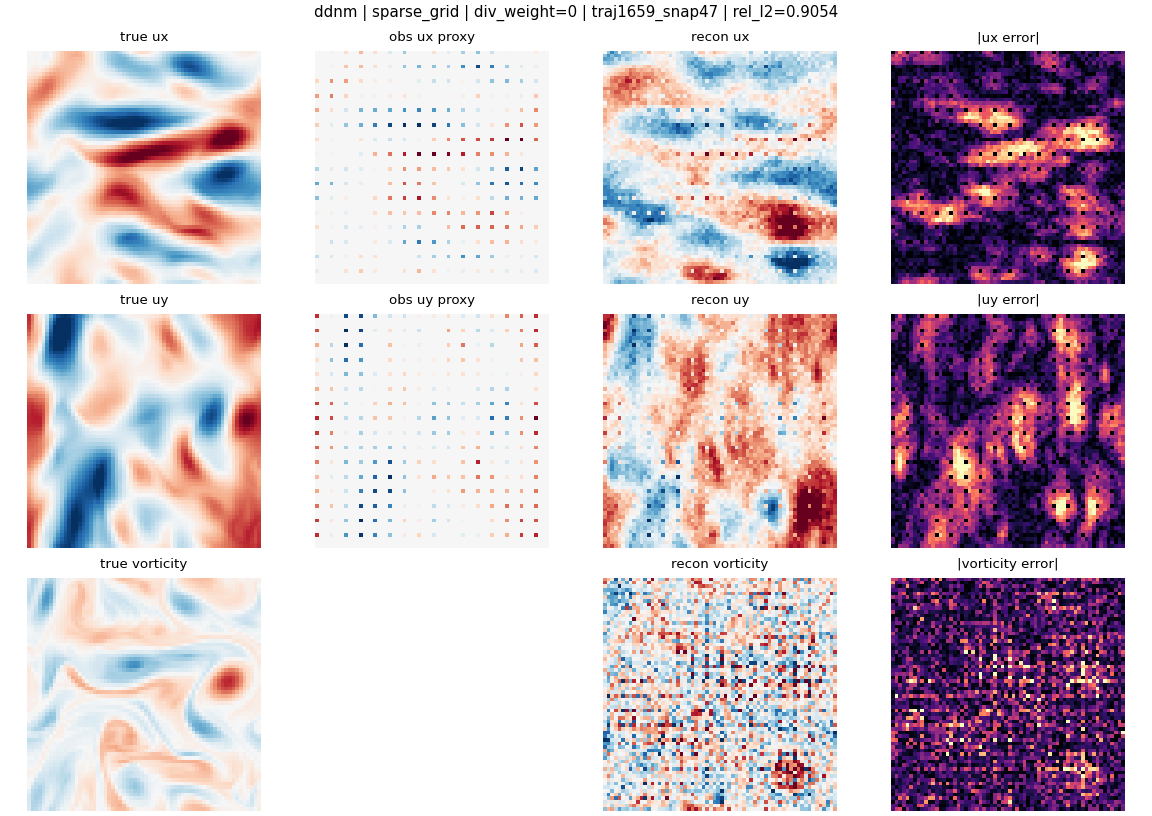
\includegraphics[width=0.47\textwidth,height=0.31\textheight,keepaspectratio]{results/ddnm_sparse.png} &
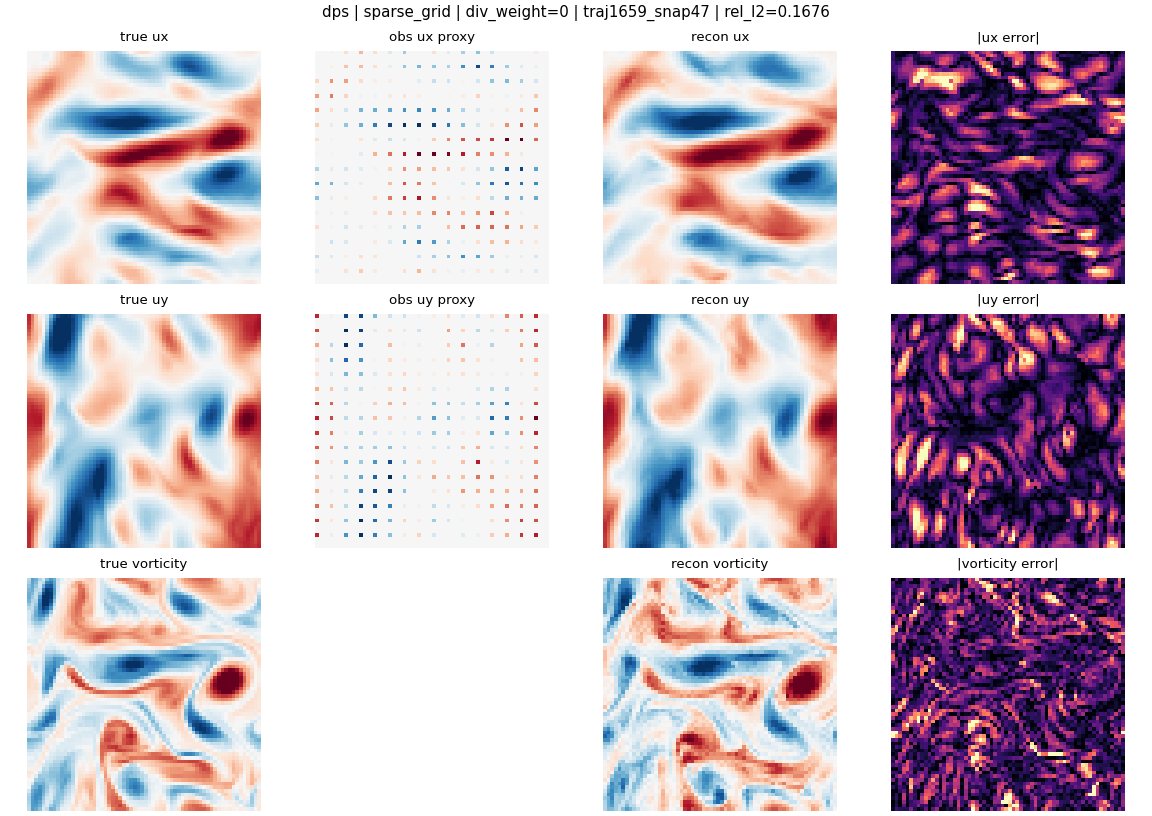
\includegraphics[width=0.47\textwidth,height=0.31\textheight,keepaspectratio]{results/dps_sparse.png} \\
\textbf{RePaint} & \textbf{DDRM} \\
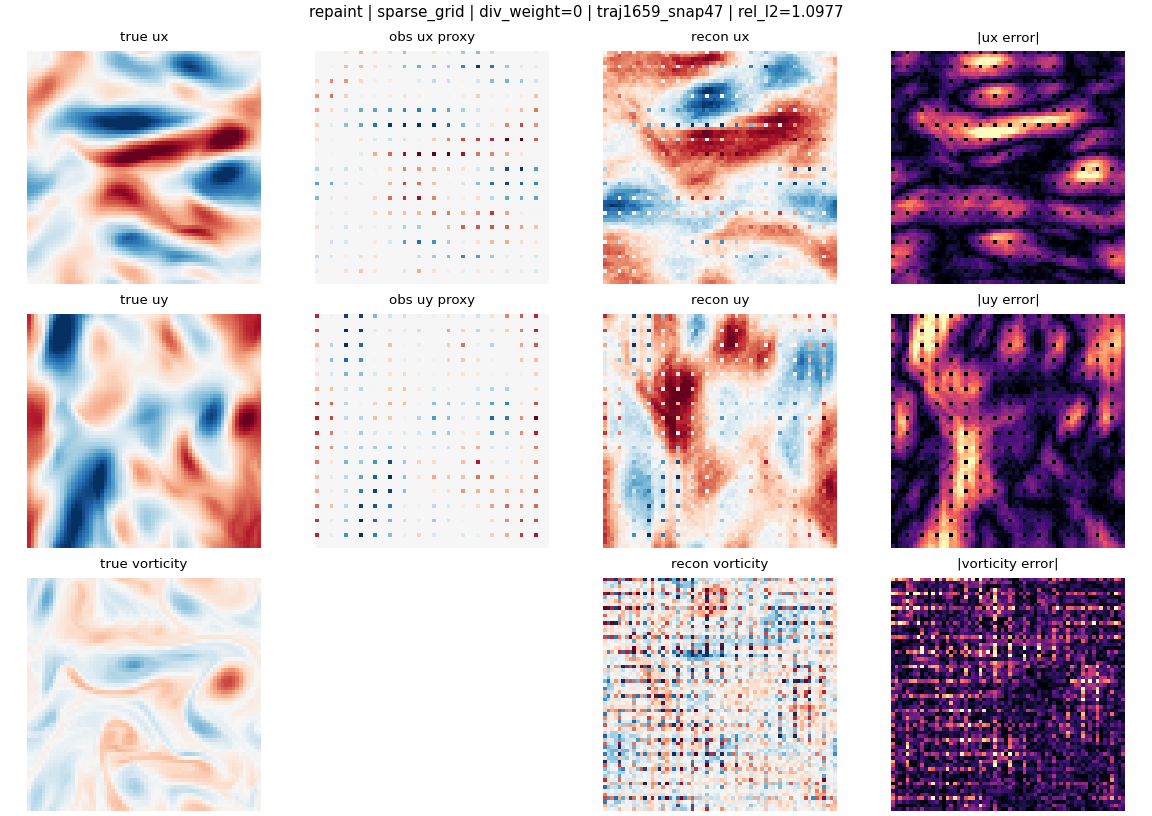
\includegraphics[width=0.47\textwidth,height=0.31\textheight,keepaspectratio]{results/repaint_sparse.png} &
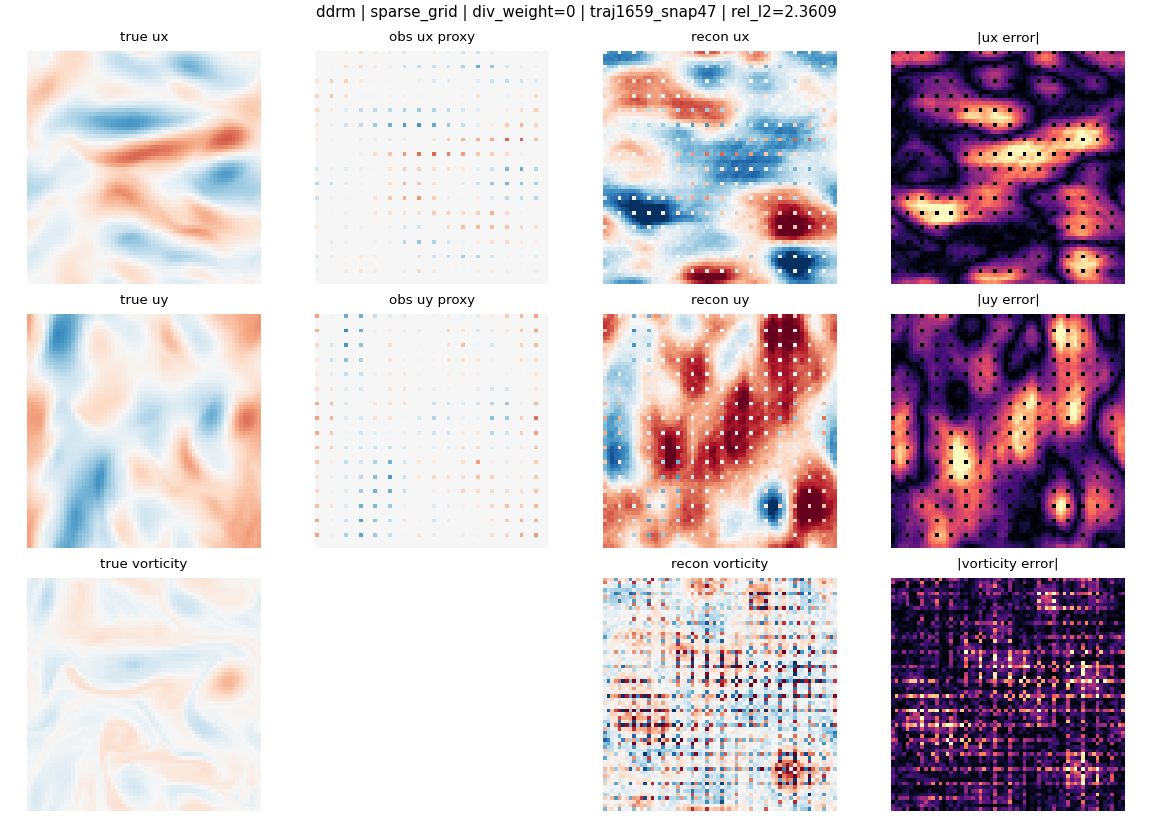
\includegraphics[width=0.47\textwidth,height=0.31\textheight,keepaspectratio]{results/ddrm_sparse.png}
\end{tabular}
\end{center}
\end{frame}

\begin{frame}{Results: Central Box Mask}
\small
Box mask $32\times32$; inner region known, outer region reconstructed. Noiseless.
\vspace{0.15cm}
\begin{center}
\begin{tabular}{cc}
\textbf{DDNM} & \textbf{RePaint} \\
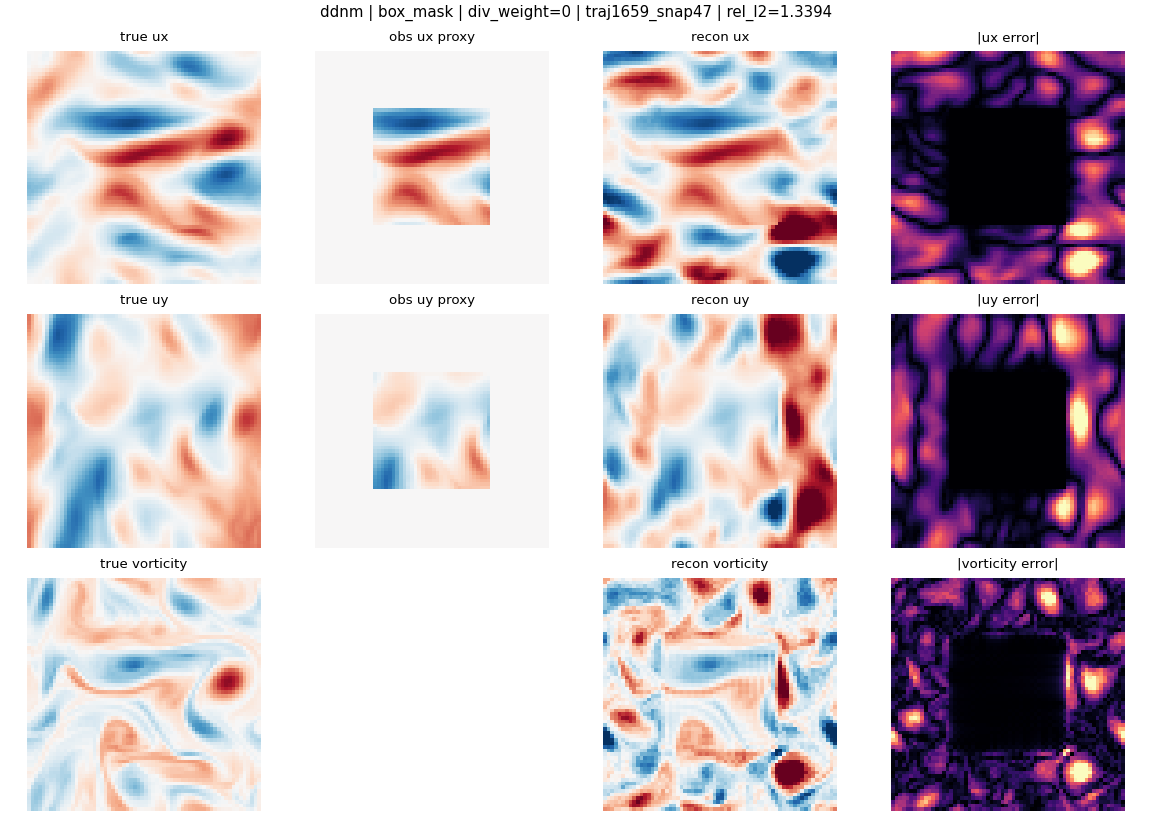
\includegraphics[width=0.46\textwidth,height=0.56\textheight,keepaspectratio]{results/ddnm_box.png} &
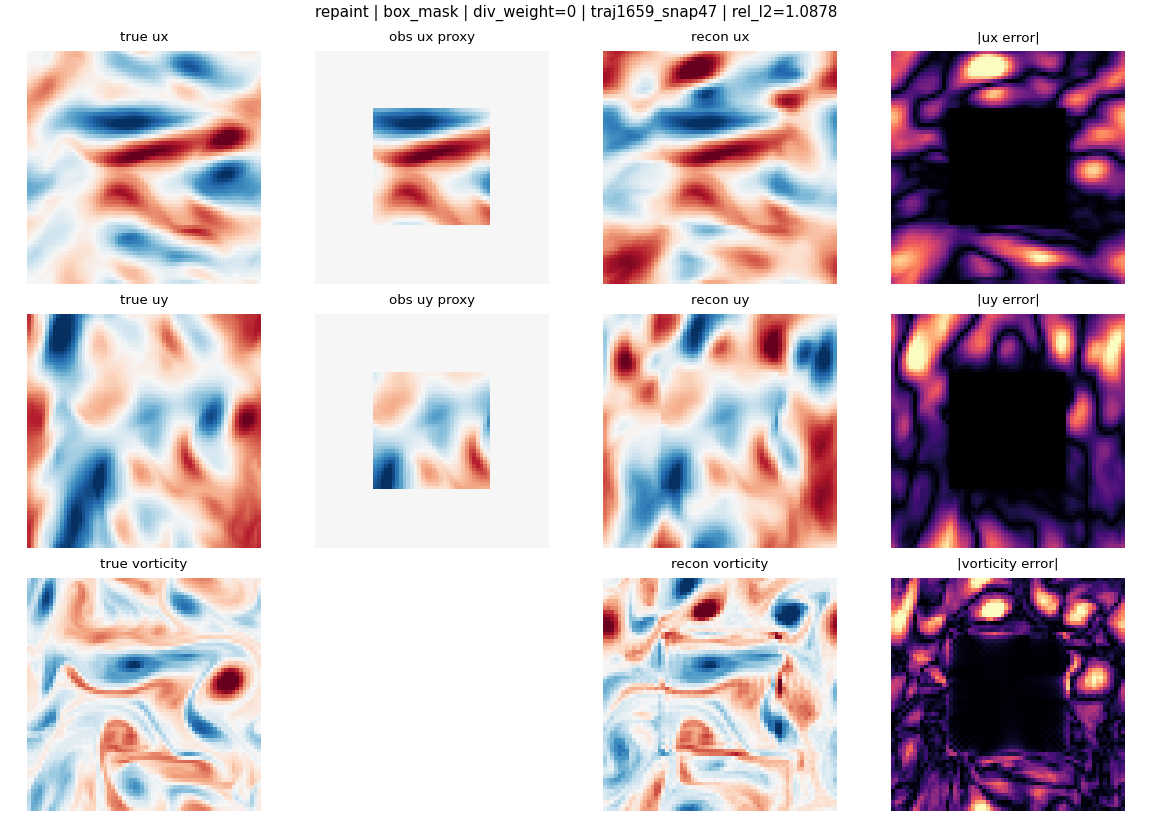
\includegraphics[width=0.46\textwidth,height=0.56\textheight,keepaspectratio]{results/repaint_box.png}
\end{tabular}
\end{center}
\end{frame}

\begin{frame}{Results: Average Downsample}
\small
$64\times64 \to 16\times16$ average pooling ($4\times$ spatial reduction). Noiseless.
\vspace{0.15cm}
\begin{center}
\begin{tabular}{ccc}
\textbf{DDNM} & \textbf{DPS} & \textbf{DDRM} \\
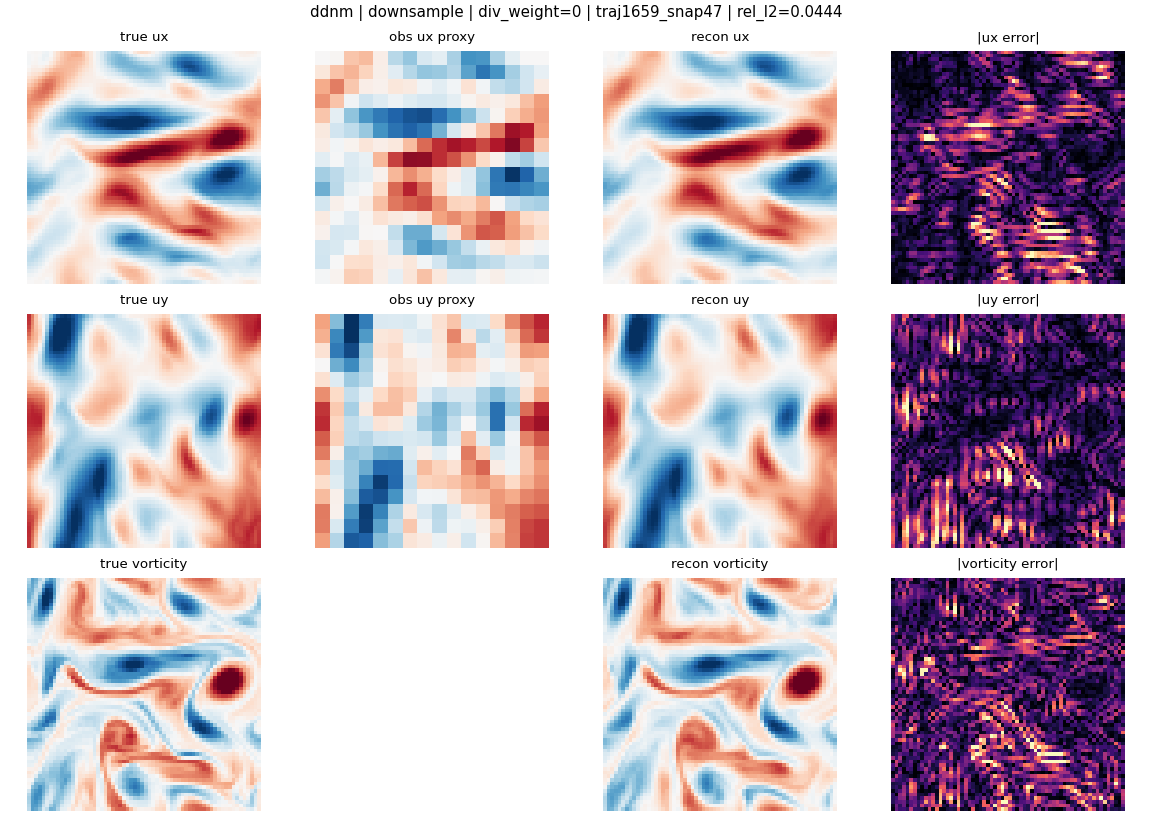
\includegraphics[width=0.29\textwidth,height=0.50\textheight,keepaspectratio]{results/ddnm_downsample.png} &
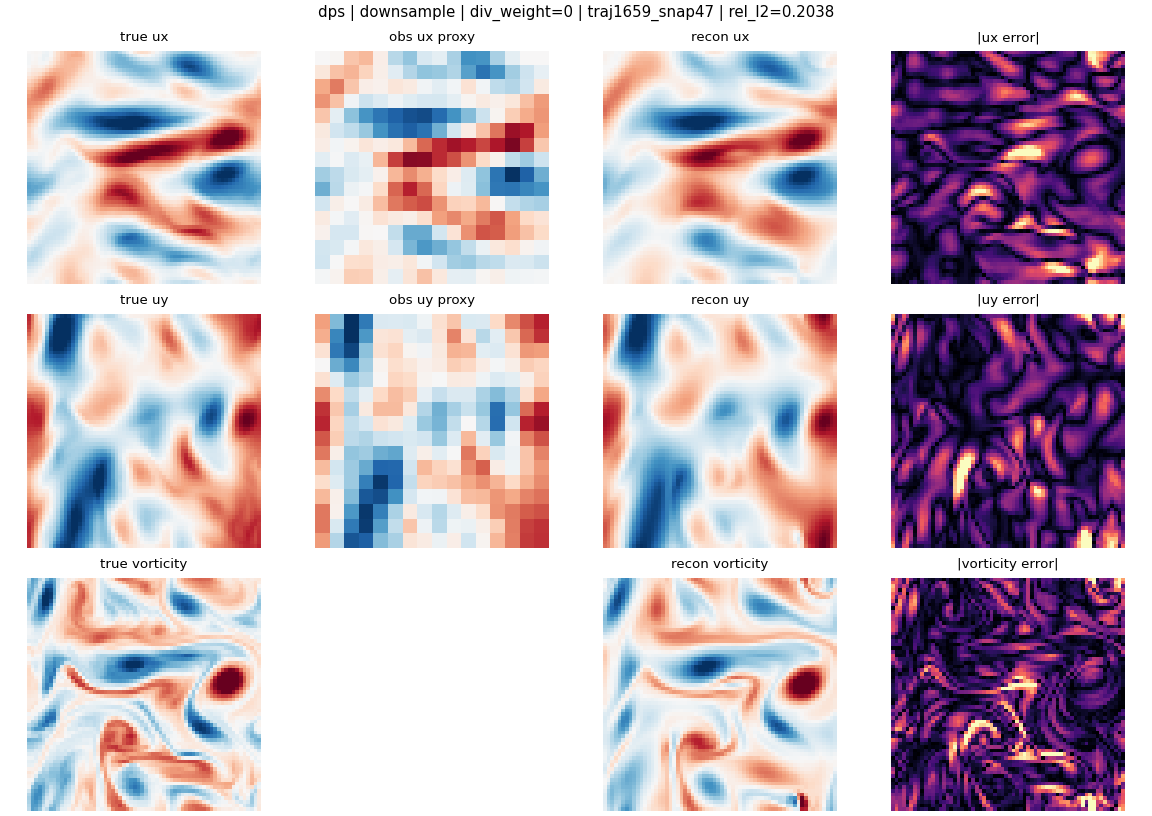
\includegraphics[width=0.29\textwidth,height=0.50\textheight,keepaspectratio]{results/dps_downsample.png} &
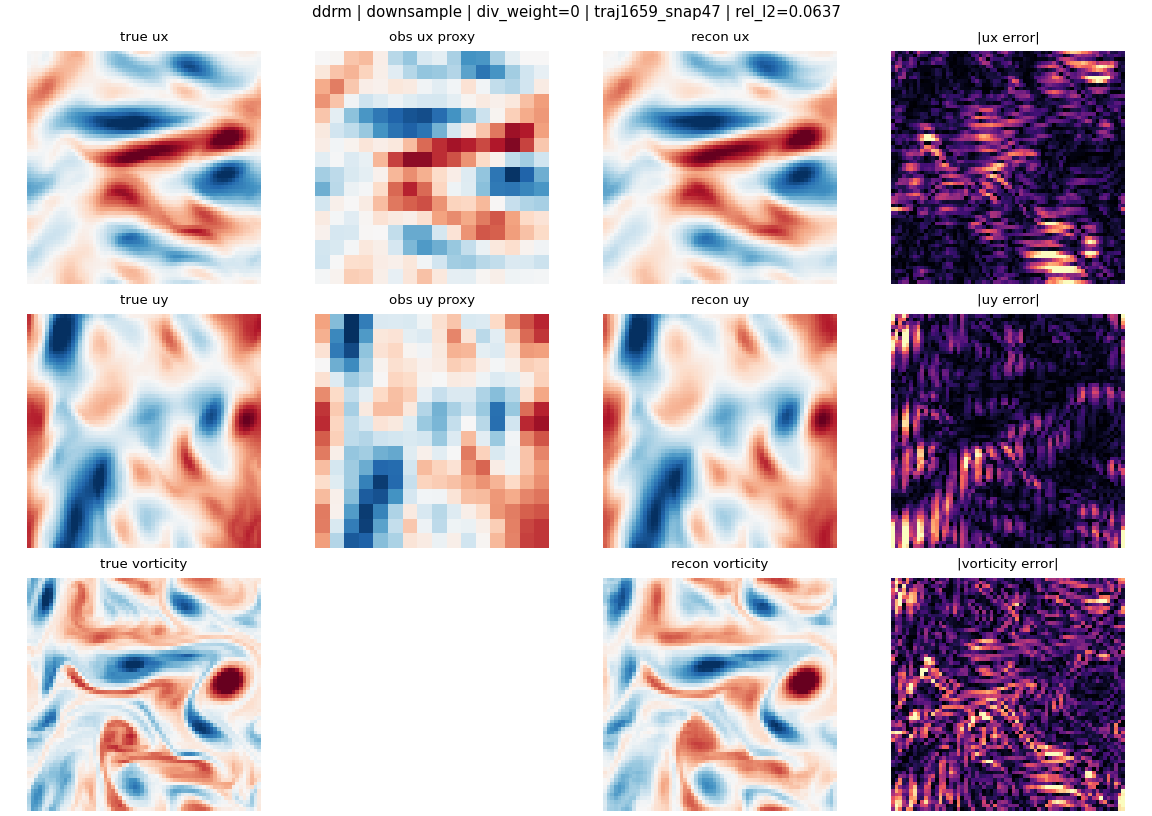
\includegraphics[width=0.29\textwidth,height=0.50\textheight,keepaspectratio]{results/ddrm_downsample.png}
\end{tabular}
\end{center}
\end{frame}

\begin{frame}{Results: Gaussian Blur}
\small
Periodic Gaussian blur with Gaussian observation noise.
\vspace{0.15cm}
\begin{center}
\begin{tabular}{ccc}
\textbf{DDNM} & \textbf{DPS} & \textbf{DDRM} \\
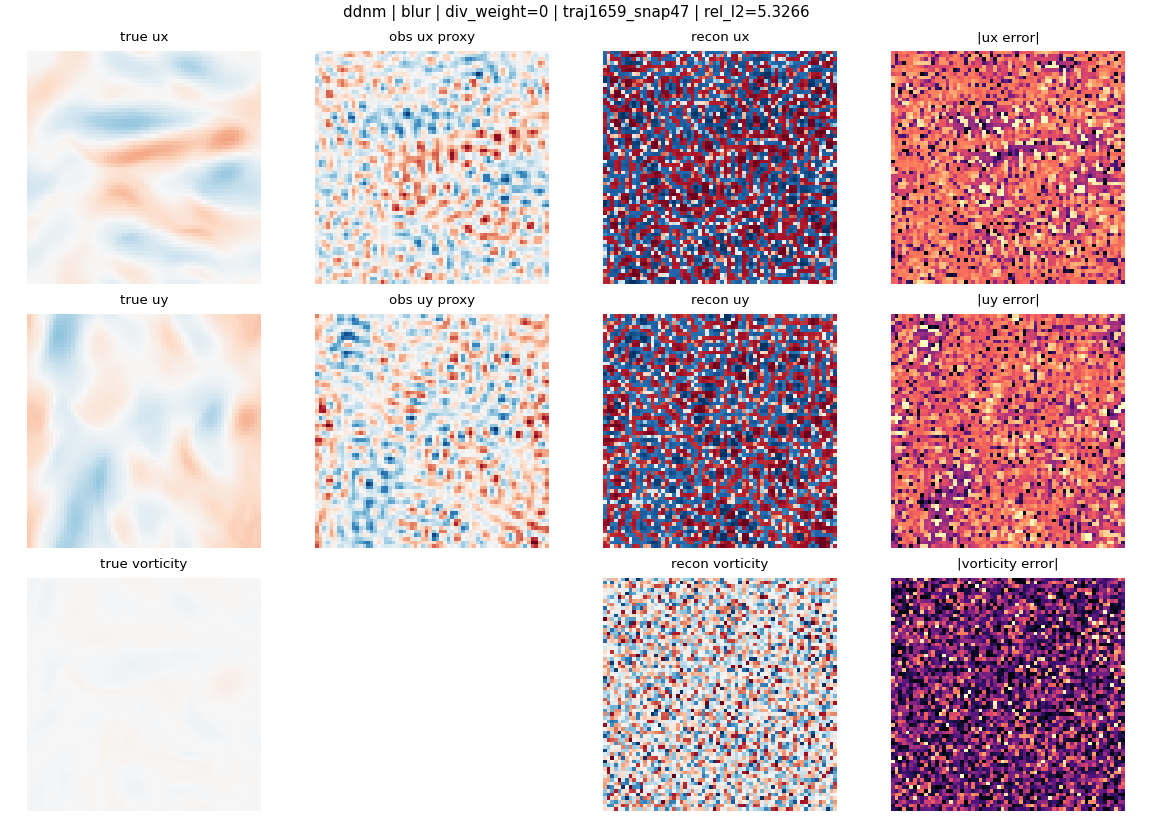
\includegraphics[width=0.29\textwidth,height=0.50\textheight,keepaspectratio]{results/ddnm_blur.png} &
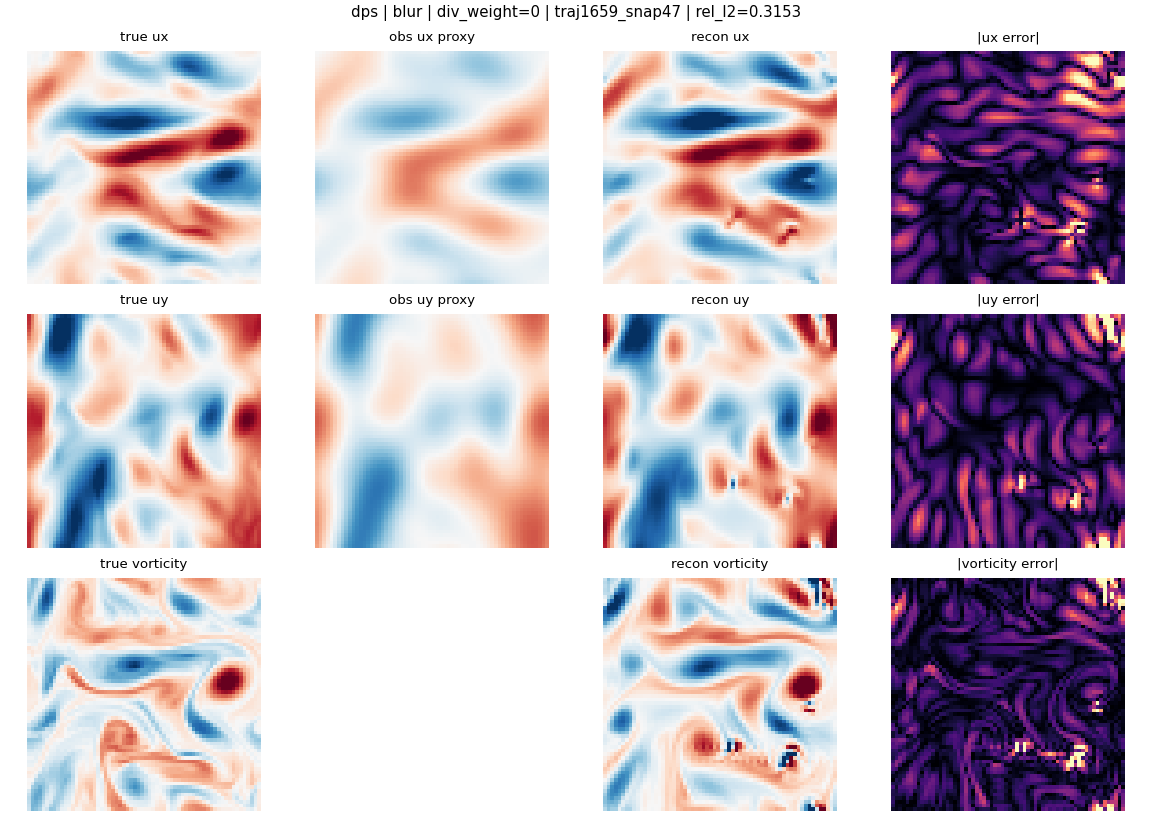
\includegraphics[width=0.29\textwidth,height=0.50\textheight,keepaspectratio]{results/dps_blur.png} &
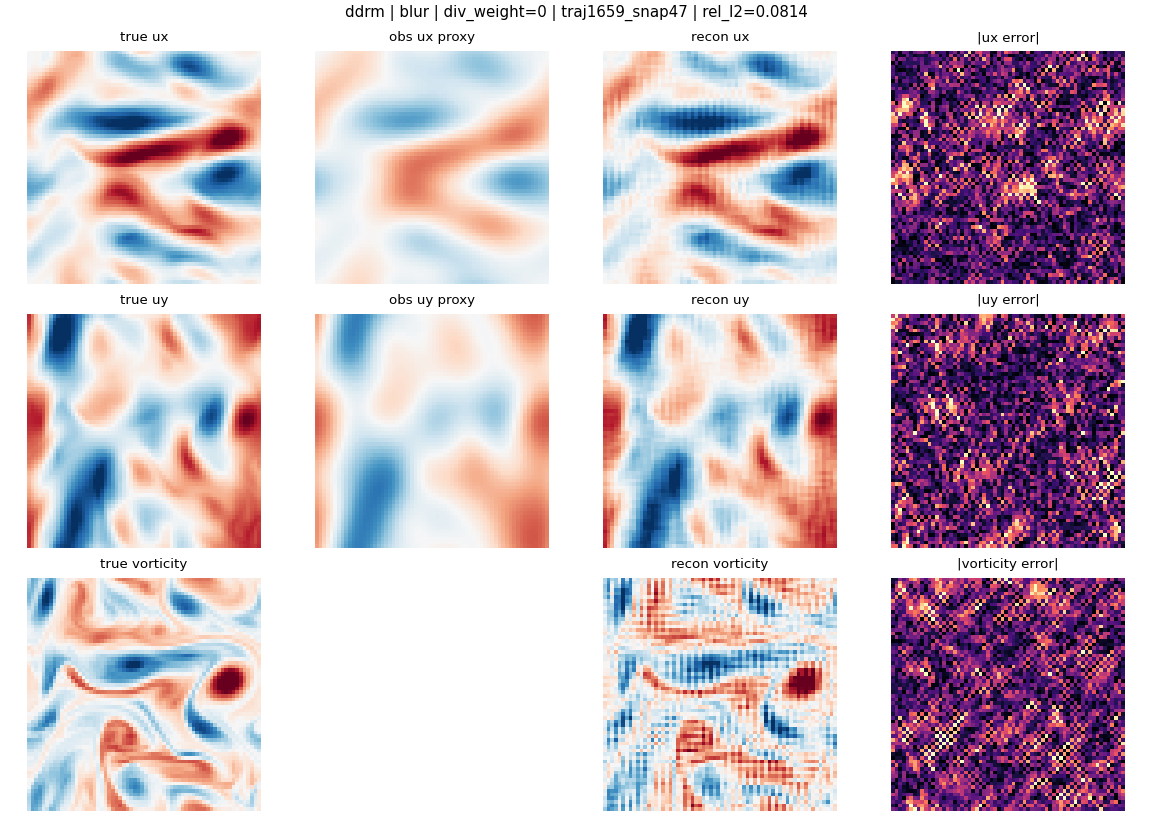
\includegraphics[width=0.29\textwidth,height=0.50\textheight,keepaspectratio]{results/ddrm_blur.png}
\end{tabular}
\end{center}
\end{frame}

\begin{frame}{Results: Quantitative Summary}
\scriptsize
\begin{center}
\resizebox{\textwidth}{!}{%
\begin{tabular}{llrrrr}
\toprule
\textbf{Operator} & \textbf{Method} & \textbf{Rel.-$L_2$} & \textbf{RMSE} & \textbf{Meas. err.} & \textbf{Divergence} \\
\midrule
Sparse grid & DDNM & 0.811 & 0.290 & $4.6{\times}10^{-4}$ & 0.523 \\
Sparse grid & DPS & 0.198 & 0.072 & $1.7{\times}10^{-1}$ & 0.038 \\
Sparse grid & RePaint & 1.188 & 0.426 & $1.9{\times}10^{-8}$ & 0.516 \\
Sparse grid & DDRM & 2.193 & 0.778 & $1.2{\times}10^{-4}$ & 0.516 \\
\midrule
Box mask & DDNM & 1.515 & 0.546 & $9.9{\times}10^{-5}$ & 0.040 \\
Box mask & RePaint & 1.434 & 0.511 & $1.9{\times}10^{-8}$ & 0.035 \\
\midrule
Downsample & DDNM & 0.050 & 0.019 & $5.9{\times}10^{-5}$ & 0.011 \\
Downsample & DPS & 0.303 & 0.107 & $2.7{\times}10^{-1}$ & 0.004 \\
Downsample & DDRM & 0.066 & 0.025 & $3.2{\times}10^{-5}$ & 0.020 \\
\midrule
Blur & DDNM & 6.132 & 2.183 & $1.4{\times}10^{-1}$ & 1.958 \\
Blur & DPS & 0.430 & 0.155 & $1.1{\times}10^{-1}$ & 0.010 \\
Blur & DDRM & 0.079 & 0.030 & $1.3{\times}10^{-5}$ & 0.182 \\
\bottomrule
\end{tabular}}
\end{center}
\vspace{0.05cm}
\tiny
Benchmark summaries from the four Colab notebooks; rows use matching debug runs ($N=16$).
\end{frame}

\begin{frame}{Physics Constraint: Does It Help?}
\scriptsize
\begin{center}
\resizebox{\textwidth}{!}{%
\begin{tabular}{llrrrr}
\toprule
\textbf{Operator} & \textbf{Method} & \textbf{Div. base} & \textbf{Div. phys.} & \textbf{Rel.-$L_2$ base} & \textbf{Rel.-$L_2$ phys.} \\
\midrule
Sparse grid & DDNM & 0.523 & 0.004 & 0.811 & 0.325 \\
Sparse grid & DPS & 0.038 & 0.026 & 0.198 & 0.198 \\
Sparse grid & RePaint & 0.516 & 0.058 & 1.188 & 0.501 \\
Sparse grid & DDRM & 0.516 & 0.095 & 2.193 & 2.174 \\
\midrule
Box mask & DDNM & 0.040 & 0.004 & 1.515 & 1.479 \\
Box mask & RePaint & 0.035 & 0.009 & 1.434 & 1.022 \\
\midrule
Downsample & DDNM & 0.011 & 0.001 & 0.050 & 0.049 \\
Downsample & DPS & 0.004 & 0.014 & 0.303 & 0.234 \\
Downsample & DDRM & 0.020 & 0.001 & 0.066 & 0.080 \\
\midrule
Blur & DDNM & 1.958 & 0.041 & 6.132 & 4.999 \\
Blur & DPS & 0.010 & 0.007 & 0.430 & 0.455 \\
Blur & DDRM & 0.182 & 0.006 & 0.079 & 0.059 \\
\bottomrule
\end{tabular}}
\end{center}
\vspace{0.15cm}
\footnotesize
Helmholtz projection consistently reduces divergence for DDNM, RePaint, and DDRM. DPS is already close to divergence-free on the debug runs; its physics term mainly changes the reconstruction/data-consistency trade-off.
\end{frame}

% ─────────────────────────────────────────────────────────────

\begin{frame}{DPS: Physics Constraint --- Visual Effect}
\small
Sparse grid operator, same sample. \textbf{Top}: with Helmholtz divergence-free penalty
(\texttt{div\_weight}\,$>0$) --- smooth, physically consistent reconstruction.
\textbf{Bottom}: without physics constraint --- visible block-like artefacts appear
in the vorticity field where the gradient guidance overfits to measurement noise.
\vspace{0.2cm}
\begin{center}
  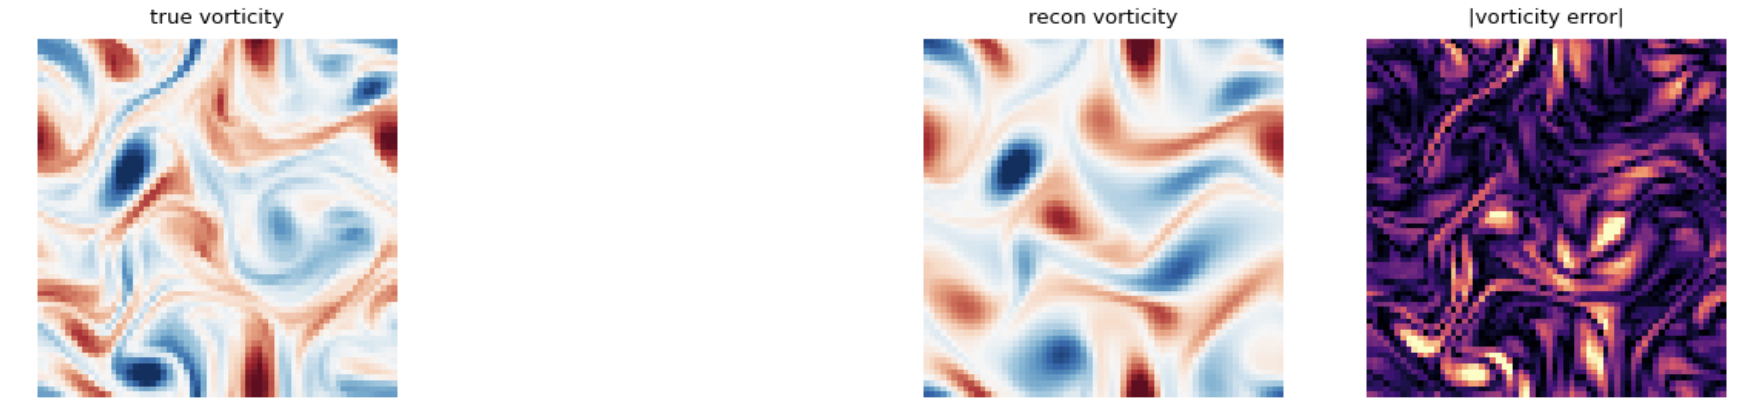
\includegraphics[width=\textwidth,height=0.34\textheight,keepaspectratio]{results/dps_physics_vorticity.png}\\[4pt]
  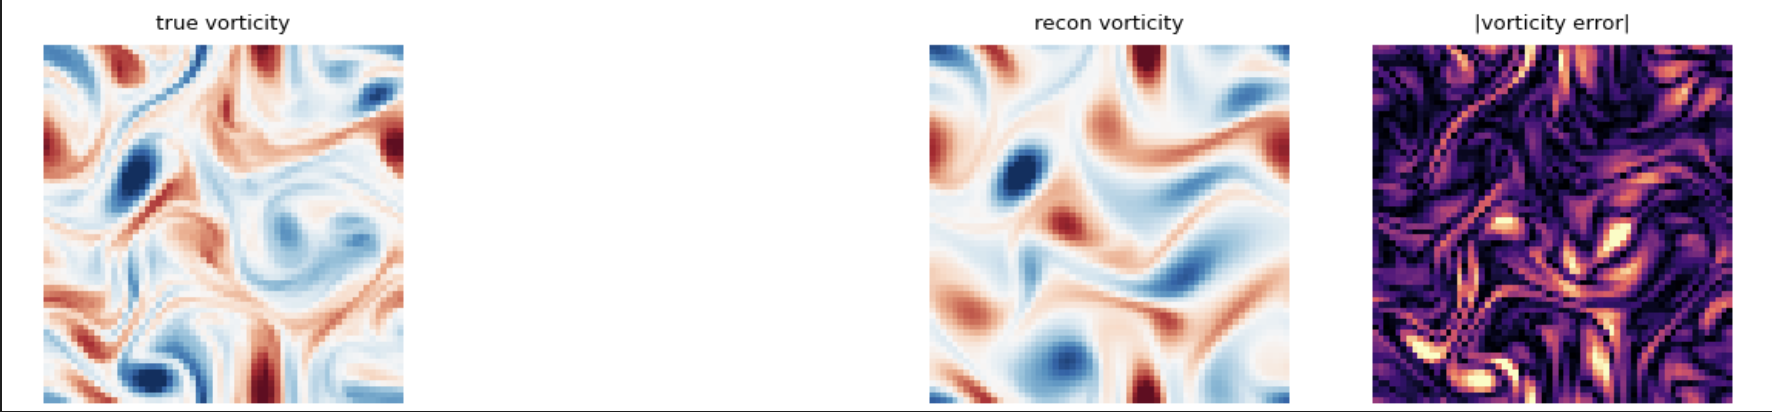
\includegraphics[width=\textwidth,height=0.34\textheight,keepaspectratio]{results/dps_no_physics_vorticity.png}
\end{center}
\end{frame}

\section{Conclusion}
% ═════════════════════════════════════════════════════════════

\begin{frame}{Conclusion}
\begin{block}{Summary}
\begin{itemize}
  \item Diffusion models provide a powerful data-driven prior for physical field reconstruction.
  \item Four zero-shot conditional sampling methods were implemented and compared
        across four observation operators on Kolmogorov flow.
  \item \textbf{DPS} is the most versatile: applicable to all operators, no pseudoinverse needed.
  \item \textbf{DDRM} is most suitable for spectral operators (blur, downsample) due to efficient
        per-frequency updates.
  \item \textbf{Helmholtz projection} provides a free improvement in physical consistency
        with minimal reconstruction penalty.
\end{itemize}
\end{block}
\begin{block}{Limitations and future work}
\begin{itemize}
  \item All methods assume the score model is well-trained on in-distribution data.
  \item Physics projection is applied post-hoc; joint training of physics-aware score models
        could improve consistency further.
  \item Extension to 3D fields and time-dependent reconstruction is a natural next step.
\end{itemize}
\end{block}
\end{frame}

% ─────────────────────────────────────────────────────────────

\begin{frame}{References and Contributions}

\begin{block}{Contributions}
\begin{tabular}{ll}
Mariia Abdullaeva & RePaint \\
Andrei Efimov & DDNM \\
Anton Losev & DDRM \\
Amir Sadreev & model training and DPS sampler \\
\end{tabular}
\end{block}
\vspace{0.1cm}

\scriptsize
\begin{enumerate}
  \item H. Chung, J. Kim, M. T. Mccann, M. L. Klasky, J. C. Ye.
        \textit{Diffusion Posterior Sampling for General Noisy Inverse Problems.}
        ICLR 2023.
  \item B. Kawar, M. Elad, S. Ermon, J. Song.
        \textit{Denoising Diffusion Restoration Models.}
        NeurIPS 2022.
  \item F. Rozet, G. Louppe.
        \textit{Score-Based Data Assimilation.}
        NeurIPS 2023.
  \item J. Song, C. Meng, S. Ermon.
        \textit{Denoising Diffusion Implicit Models.}
        ICLR 2021.
  \item A. Lugmayr, M. Danelljan, A. Romero, F. Yu, R. Timofte, L. Van Gool.
        \textit{RePaint: Inpainting using Denoising Diffusion Probabilistic Models.}
        CVPR 2022.
  \item Y. Wang, J. Yu, J. Zhang.
        \textit{Zero-Shot Image Restoration Using Denoising Diffusion Null-Space Model.}
        ICLR 2023.
\end{enumerate}
\end{frame}

% ─────────────────────────────────────────────────────────────

\end{document}
